%=== INTRODUCTION ===
%Introduction provides background information explaining the theory, processes, aims or hypothesis and rationale for conducting the research project. 

\chapter{1. Giới thiệu tổng quan về Design Pattern}
Trong kĩ thuật phần mềm, \textbf{Design Pattern} là giải pháp chung có thể lặp lại cho những vấn đề thường xảy ra khi thiết kế phần mềm. Design Pattern không phải là một thiết kế hoàn chỉnh mà chuyển hóa trực tiếp thành code. Nó là một khuôn mẫu được đúc kết từ những người đi trước nhằm giải quyết vấn đề mà có thể được sử dụng trong những trường hợp khác nhau

\section{Lợi ích của Design Pattern}
Design Pattern có thể tăng tốc quá trình phát triển bằng cách cung cấp các mô hình phát triển đã được kiểm nghiệm, chứng minh. Thiết kế phần mềm hiệu quả đòi hỏi các vấn đề đáng kể có thể không hiện hữu cho đến bước triển khai sau này. Việc sử dụng lại các design pattern giúp ngăn chặn các vấn đề nghiêm trọng và cải thiện kĩ năng đọc code cho lập trình viên và kiến trúc sư quen thuộc với các pattern\\[0.1in]
Thông thường, mọi người chỉ hiểu cách để áp dụng một số kĩ thuật thiết kế phần mềm vào những vấn đề nhất định. Những kĩ thuật này khó để áp dụng với những vấn đề ở tầm rộng hơn. Design Pattern cung cấp một giải pháp chung mà không bị bó chặt trong hoàn cảnh cụ thể nào \\[0.1in]
Hơn nữa, các design pattern dần được cải tiến theo thời gian, làm chúng trở nên mạnh mẽ hơn so với các thiết kế đặc biệt

\section{Creational design pattern}
\begin{figure}[!htb]
    \centering
    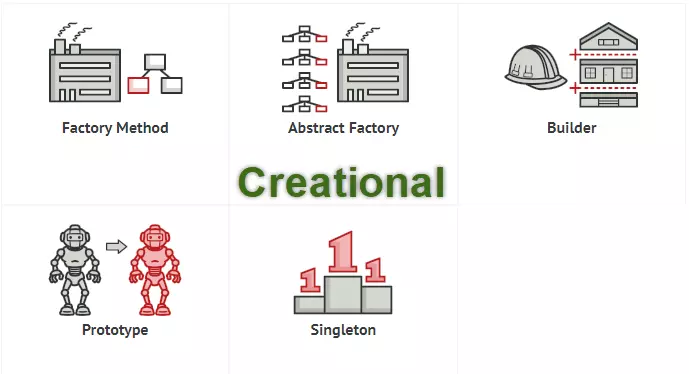
\includegraphics[width=\textwidth]{fig/Introduction/creational.png}
\end{figure}\newpage
Những design pattern này có thiên hướng khởi tạo lớp:
\begin{itemize}
    \item \textbf{Abstract Factory}: Tạo thực thể cho một số họ của các lớp
    \item \textbf{Builder}: Tách biệt cách dựng đối tượng và đối tượng được tạo ra
    \item \textbf{Factory Method}: Tạo thực thể cho mốt số lớp dẫn xuất
    \item \textbf{Object Pool}: Kiểm soát tài nguyên bằng việc tái sử dụng những đối tượng không dùng đến nữa
    \item \textbf{Prototype}: Một thực thể được khởi tạo đầy đủ được dùng để sao chép hoặc nhân bản
    \item \textbf{Singleton}: Một lớp mà chỉ một instance duy nhất có thể tồn tại
\end{itemize}

\section{Structural design patterns}
\begin{figure}[!htb]
    \centering
    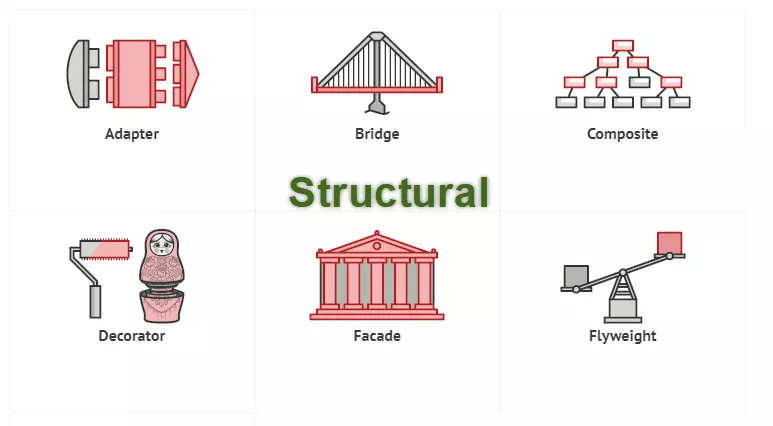
\includegraphics[width=\textwidth]{fig/Introduction/structural.png}
\end{figure}
Những design pattern này có thiên hướng liên kết giữa lớp và đối tượng với nhau:
\begin{itemize}
    \item \textbf{Adapter}: Kết nối Interface của nhiều lớp khác nhau
    \item \textbf{Bridge}: Tách biệt Interface của đối tượng với cách mà nó được triển khai
    \item \textbf{Composite}: Một cấu trúc cây của các đối tượng đơn giản và đối tượng composite
    \item \textbf{Decorator}: Thêm hành vi cho các đối tượng một cách linh động
    \item \textbf{Facade}: Một lớp đơn lẻ đại diện cho cả một hệ thống con
    \item \textbf{Flyweight}: Tái sử dụng đối tượng tương tự đã tồn tại để tối ưu bộ nhớ
    \item \textbf{Proxy}: Một đối tượng đại diện cho một đối tượng khác
\end{itemize}

\section{Behavioral design patterns}
\begin{figure}[!htb]
    \centering
    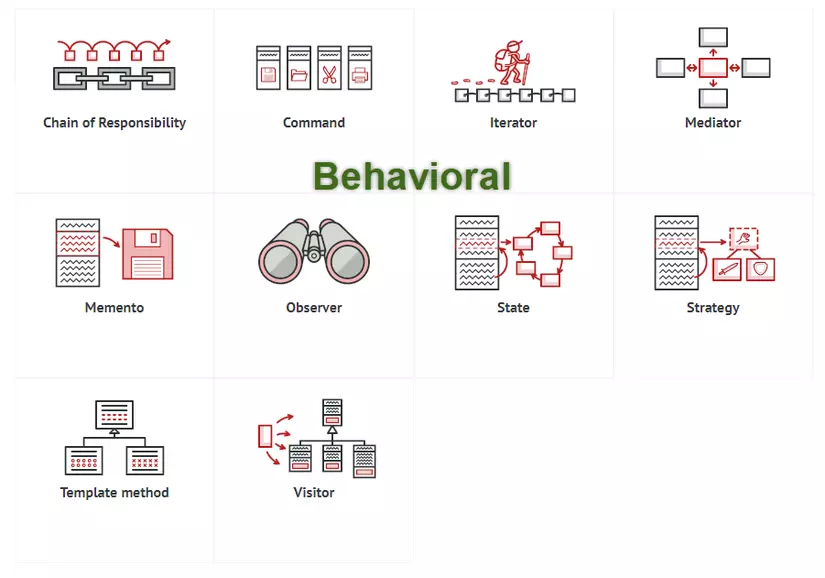
\includegraphics[width=\textwidth]{fig/Introduction/behavioral.png}
\end{figure}
Những design pattern này có thiên hướng giao tiếp giữa các đối tượng
\begin{itemize}
    \item \textbf{Chain of responsibility}: Một cách truyền yêu cầu tới một chuỗi các đối tượng
    \item \textbf{Command}: Đóng gói một lệnh dưới dạng một đối tượng
    \item \textbf{Interpreter}: Một cách để bao gồm các yếu tố ngôn ngữ trong chương trình
    \item \textbf{Iterator}: Truy cập tuần tự các phần tử của một tập hợp
    \item \textbf{Mediator}: Định nghĩa cách giao tiếp đơn giản giữa các lớp
    \item \textbf{Memento}: Lưu giữ và khôi phục trạng thái bên trong của đối tượng
    \item \textbf{Null Object}: Thiết kế để hoạt động như một giá trị mặc định của một đối tượng
    \item \textbf{Observer}: Một cách để thông báo sự thay đổi tới một số lớp
    \item \textbf{State}: Thay đổi hành vi đối tượng khi trạng thái của nó thay đổi
    \item \textbf{Strategy}: Đóng gói một thuật toán bên trong một lớp
    \item \textbf{Template method}: Trì hoãn các bước chính xác của thuật toán cho một lớp con
    \item \textbf{Visitor}: Định nghĩa các thao tác tới một lớp mà không làm thay đổi
\end{itemize}


%=== END OF INTRODUCTION ===
\newpage


